%% ACM Transactions on Embedded Computing Systems (TECS)
%% Small Standard Format (acmsmall) submission version.
%% Converted from the original IEEEtran manuscript.
\documentclass[acmsmall,review]{acmart}
\microtypesetup{expansion=false}
\setlength{\emergencystretch}{2em}

%% ---- Journal metadata (TECS) ----
\acmJournal{TECS}
\acmYear{2026}
\acmVolume{0}
\acmNumber{0}
\acmArticle{0}
\acmMonth{0}
%% For a submission, DOI/ISBN/price are assigned by ACM; defaults are fine.

%% Numeric citations (ACM small standard uses numbered references).
\citestyle{acmnumeric}

%% ---- Packages not already provided by acmart ----
\usepackage{pifont}      % \ding{...} symbols
\usepackage{makecell}    % \makecell in tables
\usepackage{subcaption}  % subfigures
% Note: acmart already provides amsmath, amssymb, graphicx, booktabs,
% xcolor, hyperref, url, caption, and natbib. Do not re-load these.

%% ---- Helper macros ----
\newcommand{\RUNTIME}{modern runtime}

\begin{document}

%% ---- Front matter (must precede \maketitle in acmart) ----
\title{Heap Memory Safeguard for Garbage Collection and Memory Management on Mobile Devices}

\author{Geunsik Lim}
\orcid{0000-0003-1845-7132}
\affiliation{%
  \institution{Sungkyunkwan University}
  \department{Department of Electrical and Computer Engineering}
  \streetaddress{2066 Seobu-ro, Jangan-gu}
  \city{Suwon}
  \postcode{16419}
  \country{South Korea}
}
\email{leemgs@g.skku.edu}

%% Short author string for running heads.
\renewcommand{\shortauthors}{G. Lim}

\begin{abstract}
Interactive latency and memory-pressure stalls on modern mobile and embedded platforms arise from a structural mismatch: applications run on a managed runtime that governs a Java heap through garbage collection, while large native (C/C++) components allocate on an unmanaged heap that the runtime cannot see, and the kernel reclaims memory page-by-page from fault addresses without any notion of application-level heap intent. We characterize this mismatch empirically on commercial devices and isolate two root causes: a \emph{visibility gap}, in which the Android Runtime (ART) is unaware of native heap growth until a physical page fault forces a reaction, and a \emph{temporal gap}, in which runtime garbage collection and kernel reclamation act reactively and at different moments, so intervention arrives after pressure has already built. Guided by these observations, we present the Heap Memory Safeguard (HMS), an OS-level framework that co-locates runtime heap telemetry with kernel-level reclamation under a single coordinated control loop. The core of HMS is a heap-utilization index $H_u$ that fuses resident footprint with allocation velocity, allowing the system to distinguish transient bursts from sustained growth and to trigger \emph{targeted} reclamation before pressure escalates---rather than uniformly reclaiming more aggressively. HMS requires no application changes and reuses standard runtime, memcg, and hardware-tagging interfaces. On two commercial smartphones across camera, gaming, on-device inference, and multitasking workloads, HMS improves heap stability, shortens garbage-collection pauses, and lowers reclaim latency relative to runtime-only and kernel-only baselines, and our analysis attributes these gains to cross-layer coordination rather than to increased reclaim aggressiveness alone.
\end{abstract}

%% ---- CCS concepts (regenerate with the official ACM CCS tool before final submission) ----
\begin{CCSXML}
<ccs2012>
   <concept>
       <concept_id>10011007.10011006.10011050.10011017</concept_id>
       <concept_desc>Software and its engineering~Garbage collection</concept_desc>
       <concept_significance>500</concept_significance>
   </concept>
   <concept>
       <concept_id>10011007.10011006.10011050.10011051</concept_id>
       <concept_desc>Software and its engineering~Allocation / deallocation strategies</concept_desc>
       <concept_significance>500</concept_significance>
   </concept>
   <concept>
       <concept_id>10011007.10011074.10011099</concept_id>
       <concept_desc>Software and its engineering~Operating systems</concept_desc>
       <concept_significance>300</concept_significance>
   </concept>
   <concept>
       <concept_id>10010583.10010588.10010589</concept_id>
       <concept_desc>Computer systems organization~Embedded software</concept_desc>
       <concept_significance>300</concept_significance>
   </concept>
</ccs2012>
\end{CCSXML}

\ccsdesc[500]{Software and its engineering~Garbage collection}
\ccsdesc[500]{Software and its engineering~Allocation / deallocation strategies}
\ccsdesc[300]{Software and its engineering~Operating systems}
\ccsdesc[300]{Computer systems organization~Embedded software}

\keywords{Heap memory, memory management, garbage collection, cross-layer
coordination, mobile operating systems, Android runtime, kernel reclamation,
on-device inference}
   % abstract + CCS concepts + keywords

\maketitle

%% ---- Body ----
\section{Introduction}
Mobile and embedded platforms such as smartphones, portable media players, and tablets have repeatedly been shown to suffer poor user experience from memory pressure, fragmentation, and wasteful reclamation~\cite{TCE_Lim2013_VMP, TC_10492614}. In a managed runtime, the region of memory that stores application objects is the \textit{heap}; it is grown and shrunk automatically by the allocator, and object reclamation is delegated to a garbage collector rather than to explicit deallocation. Modern Android systems address heap pressure by combining the Android Runtime (ART) with compacting generational garbage collection, compressed-memory mechanisms such as zRAM, and kernel-level controls originally explored in embedded and virtualized devices~\cite{TCE_Hwang2012_CompressedSwap, TC_9140304, TC_10851391}. Despite these mechanisms, heap footprint still grows in ways the runtime cannot anticipate, because native (C/C++) libraries reached through the Java Native Interface (JNI)---for example, media, graphics, and inference frameworks---allocate outside the managed heap and are therefore invisible to ART's accounting. This unmanaged growth is a major cause of latency spikes, forced termination of background processes, and performance degradation under load.

Modern mobile devices thus combine a managed Java heap under the runtime with an unmanaged native heap accessed through C/C++ libraries. This dual-heap architecture reflects long-standing trade-offs between performance and control in general-purpose and embedded computing~\cite{TCE_Shin2010_FTL,TC_9252863}. While the runtime reclaims Java objects through concurrent garbage collection, native allocations remain largely opaque to it, producing asymmetric visibility and delayed response under sustained workloads such as real-time media processing, interactive graphics, and on-device inference~\cite{TC_9513533}. As pressure builds, kernel-level reclaim and swap are triggered, frequently causing excessive reclamation overhead and unpredictable application behavior~\cite{TC_10851391}.

Earlier Android generations already shifted heap-management responsibility from application developers to the managed runtime, mirroring trends across mobile and embedded consumer platforms. Runtime-centric regulation, however, is fundamentally \emph{reactive}: ART begins collecting only after a generation threshold is crossed, and the kernel begins reclaiming only after page-level pressure is detected, so both mechanisms respond to overshoot rather than preventing it. Although Linux cgroup controllers and memory limits provide isolation, they lack semantic awareness of application-level heap dynamics, especially when multiple libraries share memory pages. This mismatch between kernel-level reclamation and runtime accounting often results in premature process termination or repeated garbage-collection cycles~\cite{TCE_Kim2018_QoS, TC_11313797}. The problem is intensified by on-device intelligence, where memory behavior interacts tightly with inference pipelines, on-device learning, and adaptive workloads~\cite{TCE_Protogeros2025_FL,TC_10564838}; existing approaches, however, optimize mainly for computational or communication efficiency and do not integrate heap growth and reclamation into a single OS-level control loop.

\smallskip
\noindent\textbf{Positioning.} We group prior memory-management work into three families and state up front how HMS differs from each. \emph{Runtime-level} techniques adapt garbage collection to allocation patterns~\cite{TC_10045641,TCE_Yan2019_FileAwareGC} but reason only about managed objects and cannot see native growth. \emph{Kernel-level} techniques reclaim and compress pages~\cite{TCE_Hwang2012_CompressedSwap,TC_9140304,TC_9513533} but act on physical pages without object- or heap-level semantics. \emph{Hardware-assisted} mechanisms such as ARM Memory Tagging detect memory-safety errors but do not regulate heap growth. A few recent efforts coordinate across tiers for edge and cloud inference~\cite{TC_10320372,TCE_Wang2025_CloudEdge}, yet they prioritize network efficiency and latency rather than heap stability. HMS differs by making the runtime's logical view of heap growth and the kernel's physical reclaim actuators \emph{observe and act through one shared control loop}, so that reclamation is both semantically informed and temporally aligned. Section~\ref{sec_related} contrasts these families in detail (Table~\ref{tab:related_compare}).

To close the visibility and timing gaps identified above, we propose an OS-level \textbf{Heap Memory Safeguard (HMS)} that coordinates heap control across the runtime and kernel layers. We first analyze empirical, cross-layer characteristics of heap behavior on commercial devices to expose the persistent visibility and timing gaps between runtime garbage collection and kernel-level reclamation~\cite{TC_10492614,TC_10045641, TC_9140304}. Building on these insights, HMS bridges the kernel's physical memory view and the runtime's logical heap by monitoring allocation trends and coordinating targeted reclamation before pressure escalates. The design draws on prior work in kernel-aware compaction and workload-sensitive memory management~\cite{TCE_Lim2013_VMP,TC_9513533} and extends it to Android-class platforms through explicit cross-layer coordination. This coordination problem rarely arises in general-purpose systems: mobile and CE devices operate under strict memory budgets, often lack swap-backed virtual memory, and must sustain predictable interactive latency while continuously running tightly coupled managed and native workloads.

\smallskip
\noindent\textbf{Contributions.} This paper makes the following contributions:
\begin{enumerate}
  \item \textbf{Empirical characterization.} Using commercial devices, we quantify a \emph{visibility gap} (ART is blind to native heap growth until a page fault) and a \emph{temporal gap} (runtime and kernel act reactively and at different times), and we show that these gaps, not raw memory scarcity alone, drive interactive stalls (Section~\ref{sec_motivation}).
  \item \textbf{A fused utilization signal with an explicit rationale.} We introduce the heap-utilization index $H_u$, which combines resident footprint with allocation velocity, and we derive why this combination separates transient bursts from sustained growth better than footprint-only, rate-only, or pressure-only signals (Section~\ref{subsec_rationale}).
  \item \textbf{A cross-layer system, HMS.} We design and implement HMS---a Runtime Observer, a Kernel Enforcer, and a memcg/tagging feedback interface---that requires no application changes and reuses standard interfaces (Section~\ref{sec_hms}).
  \item \textbf{Analysis that isolates the source of the benefit.} Beyond aggregate speedups, we analyze \emph{why} HMS helps: we examine the reclaim--GC interaction, quantify control overhead and misprediction behavior, and separate the contribution of cross-layer coordination from that of merely reclaiming more aggressively (Sections~\ref{sec_eval}--\ref{sec_case}).
\end{enumerate}

\section{Background}
\subsection{Managed and Native Allocation}
ART garbage collection reasons about managed objects.  Native allocations may be
reported to the runtime through Android allocation-notification mechanisms, but
such notifications are not equivalent to ownership of native objects or complete
knowledge of allocator caches, mappings, sharing, and page residency.  Native
allocation rate is likewise not RSS growth: lifetime, frees, reuse, page
commitment, file mappings, and reclaim all intervene.  HMS consequently treats
managed allocation, sampled native allocation, and RSS as distinct observations.

\subsection{Linux and Android Memory Pressure}
Linux memory cgroups account and limit groups of processes and expose a
\texttt{memory.reclaim} interface for proactive, cgroup-scoped reclaim.  PSI means
\emph{Pressure Stall Information} and quantifies time in which tasks stall for
resources.  Android's LMKD consumes pressure and process-importance information;
zRAM provides compressed swap; MGLRU and DAMON/DAMOS provide additional
working-set and proactive-reclaim mechanisms.  HMS is a proposed trigger and
budgeting layer above these facilities, not a replacement for them.

\subsection{Memory Tagging}
Arm Memory Tagging Extension (MTE) detects classes of spatial and temporal memory
safety errors.  An MTE fault is not a normal heap-pressure signal, and this paper
does not use it as a predictor.  Production mode, overhead, causality, and fallback
would require a separate device study.  MTE is therefore outside the evaluated HMS
control path.

\section{Motivation and Scope}
\label{sec_motivation}
The motivating scenario is a hybrid application whose managed heap is stable while
native allocations and resident pages grow.  A managed-only controller may see
little reason to collect, whereas a pressure-only controller reacts after the
system is already contended and may not identify which application's recent growth
is responsible.  Combining the signals could permit an earlier and more selective
request.

This paper evaluates that proposition only in simulation.  The four workload
generators model bursty camera, game-streaming, inference, and multitasking
allocation traces.  They do not model a named application, exact camera resolution,
TensorFlow Lite model, AR scene, vendor kernel, thermal state, or background-process
population.  No numerical observation in the evaluation should be interpreted as a
commercial-device measurement.

The scope restriction is important.  A deployable study must measure observer
error and delay, allocator survival and reuse, refaults during GC, writeback, energy,
thermal behavior, application kills, and long-run oscillation.  It must also
compare equal-reclaim-volume policies and publish raw traces and every per-run
record.  Section~\ref{sec_eval} lists these requirements alongside the simulation
results so that feasibility evidence is not confused with deployment evidence.

\section{HMS Design}
\label{sec_hms}
\begin{figure}[t]
  \centering
  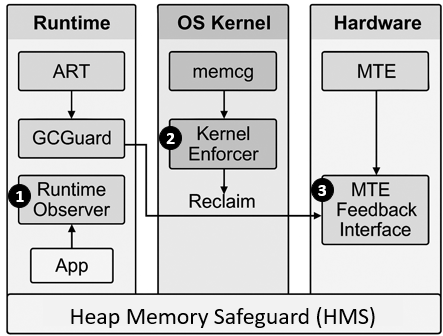
\includegraphics[width=0.85\linewidth]{./fig1_hms_architecture.png}
  \caption{Proposed HMS integration boundary.  Solid components are represented by
  the simulation; dashed Android/runtime/kernel connections are design targets.}
  \Description{Three-layer HMS concept: a user-space observer combines managed,
  native, resident, and pressure telemetry; a controller computes a reclaim
  request; and an existing memory-cgroup actuator performs bounded reclaim.  The
  repository simulates these components and does not implement Android hooks.}
  \label{fig:hms_architecture}
\end{figure}

\subsection{State Model}
For application $i$ at sample $t$, HMS records managed allocation activity
$a_i^m(t)$, sampled native allocation activity $a_i^n(t)$, RSS $R_i(t)$, the
configured memcg limit $L_i(t)$, and PSI $p_i(t)$.  The first four signals form the
controller input.  PSI is a lagging safety signal and is used to suppress additional
work during an existing severe stall, not as proof of heap ownership.

The original score is retained as an explicitly heuristic index:
\[
H_i(t)=\frac{R_i(t)}{L_i(t)}
       +\alpha\frac{\widehat{g}_i(t)}{G_i(t)} ,
\]
where $\widehat{g}_i(t)$ is an exponentially smoothed \emph{net resident-growth
estimate}, not raw object allocation, and $G_i(t)$ is an online scale.  We set
\[
G_i(t)=\max\{\epsilon,Q_{0.95}(\lvert\widehat{g}_i\rvert)
\text{ over a trailing window}\}.
\]
Only past samples enter the window; values above the current scale are clipped.
This avoids whole-experiment maxima and future-data leakage.  The score is
dimensionless, and $\alpha$ is a weight.  It is not a prediction horizon or a
calibrated time-to-pressure estimate.

For a deployable controller, a more interpretable quantity is
\[
T_i^{\mathrm{pressure}}(t)=
\frac{\max(0,L_i(t)-R_i(t))}
     {\max(\widehat{g}_i(t),\epsilon)} .
\]
The simulation retains $H_i$ to study the published lightweight policy; evaluation
of calibrated time-to-pressure error is future work.

\subsection{Control and Bounded Actuation}
Two thresholds provide hysteresis.  Crossing $\theta_1$ enters observation state;
crossing $\theta_2$ creates a reclaim request.  A request contains a cgroup
identifier, maximum byte budget, deadline class, and cooldown.  An implementation
should invoke an existing scoped actuator such as \texttt{memory.reclaim}; this
paper does not claim a \texttt{vmscan} modification, custom \texttt{GCGuard} API, or
\texttt{system\_server} service.

The budget is capped by the smaller of excess resident bytes and a per-cycle
fraction of the cgroup limit.  A cooldown prevents immediate repetition.  Refault
or rising PSI feedback reduces the next budget.  GC-active and render-deadline
windows defer reclaim unless the cgroup is at its hard limit.  These rules bound
work per cycle but do not constitute a formal stability proof.

\subsection{Concurrent Applications and Fairness}
For simultaneous requests, HMS orders foreground-deadline classes ahead of
background throughput classes and applies deficit round-robin within each class.
Each cgroup receives a token bucket proportional to its configured limit; unused
tokens carry over only to a fixed cap.  Per-cgroup and global reclaim budgets bound
one cycle.  Process exit cancels queued work, and cgroup identity must be
revalidated before actuation.  This policy prevents starvation in the model, but
priority inversion, shared-page accounting, cgroup offlining, lock contention, and
competition with direct reclaim or kswapd remain implementation questions.

\subsection{Artifact Boundary}
The Python package models telemetry, controller decisions, a memcg-like reclaim
proxy, and a tagging proxy.  It has no privileged service, Binder/eventfd path,
\texttt{heapprofd} integration, \texttt{smaps} parser, SELinux policy, or kernel
module used by the reported runs.  The historical package name \texttt{hmp} is an
import-compatibility detail.  This explicit boundary is part of the design:
simulation can test policy logic, while only a future Android implementation can
establish overhead, safety, or effectiveness on hardware.

\section{Simulation Evaluation}
\label{sec_eval}
\subsection{Questions and Method}
We ask three questions: (Q1) does the simulated two-signal controller reduce
footprint variability relative to no controller; (Q2) how sensitive are outcomes
to $\alpha$, $\theta_1$, and $\theta_2$; and (Q3) can every reported value be
regenerated from a seed and script?  We do not ask whether HMS outperforms Android
on a phone.

The artifact generates four synthetic traces: W1 (bursty camera-like allocation),
W2 (streaming game assets), W3 (inference-like tensor bursts), and W4
(multi-application switching).  A run is identified by configuration and random
seed.  The baseline and HMS consume the same generated trace.  Commands, output
schema, and provenance are documented in the repository README.  Values are
simulation units scaled for readable plots; they are not milliseconds, megabytes,
watts, or device confidence intervals unless independently calibrated.

\subsection{Metrics}
Heap stability has one definition throughout the paper and code:
\[
S_h=1-\frac{\sigma(R)}{\max(\mu(R),\epsilon)} .
\]
The evaluation window is the complete post-warm-up trace.  We report $S_h$ together
with peak RSS because a stable but large footprint should not be rewarded without a
size metric.  $L_r$ is simulated reclaim-service latency, never ``memory seek
latency.''  $T_{gc}$ is simulated pause duration.  Tail percentiles, deadline
misses, energy, and effect sizes require per-run device data and are not claimed.

\begin{figure*}[t]
\centering
\begin{subfigure}{0.42\textwidth}\centering
  
\includegraphics[width=\linewidth]{fig9_W1_alpha_vs_Sh_3alpha.png}
  \caption{W1: $\alpha$ versus $S_h$}
  \Description{A line plot of simulated W1 stability over an alpha sweep.}
\end{subfigure}\hspace{0.04\textwidth}
\begin{subfigure}{0.42\textwidth}\centering
  
\includegraphics[width=\linewidth]{fig9_W2_theta1_vs_Lr.png}
  \caption{W2: $\theta_1$ versus $L_r$}
  \Description{A line plot of simulated W2 reclaim latency over a threshold sweep.}
\end{subfigure}
\begin{subfigure}{0.42\textwidth}\centering
  
\includegraphics[width=\linewidth]{fig9_W3_theta2_vs_Sh.png}
  \caption{W3: $\theta_2$ versus $S_h$}
  \Description{A line plot of simulated W3 stability over a threshold sweep.}
\end{subfigure}\hspace{0.04\textwidth}
\begin{subfigure}{0.42\textwidth}\centering
  
\includegraphics[width=\linewidth]{fig9_W4_theta2_vs_Lr.png}
  \caption{W4: $\theta_2$ versus $L_r$}
  \Description{A line plot of simulated W4 reclaim latency over a threshold sweep.}
\end{subfigure}
\caption{Seeded simulation parameter sweeps.}
\Description{Four plots show sensitivity of simulated stability and reclaim
latency to controller weights and thresholds.}
\label{fig:parameter_sensitivity}
\end{figure*}

\subsection{Interpretation}
The simulation exposes a mixed trade-off rather than a universal improvement:
with the documented seed, controller enforcement reduces the reclaim- and
GC-service proxies and peak RSS, while $S_h$ can decrease because the bounded
interventions add footprint variation.  Parameter sweeps also show that the outcome
depends on threshold selection.  This is a sanity-check of controller logic and a
falsifiable warning against relying on a single metric, not empirical validation.
Exact numerical
claims from earlier drafts---including commercial-device p99 latency,
misprediction rate, post-reclaim faults, compatibility, CPU overhead, and
low-pressure regression---have been removed because their raw inputs are absent.

\subsection{Required Device Evaluation}
A future empirical paper must publish one row per device, workload, system, and run
with peak RSS; GC p50/p95/p99; reclaim p99; frame p99 and miss ratio; energy;
reclaim volume; refaults; and application kills.  Raw Perfetto traces,
\texttt{hms\_events.jsonl}, RSS, vmstat, PSI, configuration, exclusions, and analysis
scripts must accompany those rows.

Required baselines are stock Android, tuned LMKD/PSI, direct
\texttt{memory.reclaim}, equal-volume static reclaim, a PSI-driven userspace
daemon, DAMON/DAMOS, MGLRU tuning, footprint-only, rate-only, and signal ablations.
At least four memory tiers and two SoC vendors should be studied.  Long-duration,
energy, thermal, writeback, functional-correctness, and multi-process fairness
tests are also required.

Statistical analysis must be selected after inspecting the raw distribution.
Repeated measures should preserve pairing; device and run effects should not be
pooled as independent observations.  Bootstrap intervals or paired nonparametric
tests are appropriate for heavy-tailed metrics, with Holm correction and an effect
size such as Cliff's delta.  No t-test or confidence interval is reported here
because the repository contains no qualifying device observations.

\section{Deployment Scenarios and Validation Plan}
\label{sec_case}
Camera and inference pipelines are motivating scenarios rather than case studies.
A camera study must identify resolution, frame rate, HDR burst length, segmentation
model, tensor dimensions, correctness criterion, and background state.  An
inference or AR study must identify model, scene, tracking-quality metric, reload
behavior, and task-completion criterion.  Each must publish repetitions and
variance rather than phrases such as ``no noticeable delay.''

An Android prototype must disclose the AOSP tag, ART and kernel commits, GKI/vendor
changes, collector, heap limit, zRAM, LMKD properties, MGLRU state, root/bootloader
requirements, changed files and lines of code, service permissions, communication
path, and SELinux policy.  If a custom runtime hook is introduced, its public
contract and synchronization cost must be included; the name ``GCGuard API'' is
not used because no such implementation exists in this repository.

Compatibility must be stated narrowly as the tested application set, not as
compatibility with all Android software.  Energy and sustainability claims require
CPU, DRAM, device-power, wakeup, compression-time, thermal, and battery
measurements.  Until these experiments and artifacts exist, HMS remains a
simulation-backed design proposal.

\section{Related Work}
\label{sec_related}
Software runtimes, operating system kernels, and hardware features have all contributed to the advancement of mobile device memory management research. Here, we summarize the key issues and trends addressed in previous research.


\subsection{Runtime-Level Heap Optimization}
Virtual machines such as Dalvik and ART were at the center of the first attempts to improve memory handling in mobile environments. Reducing garbage collection latency and memory fragmentation without exceeding the limited memory capacity of mobile devices has been an ongoing challenge for developers. Recent adaptive garbage collection techniques \cite{TC_10045641,TCE_Yan2019_FileAwareGC}, which adjust their behavior according to workload patterns, have made considerable progress in this area. These strategies, along with the introduction of concurrent and generational garbage collectors, have helped reduce pause times. However, in applications currently heavy in multimedia and AI workloads, a significant portion of native memory allocations are primarily confined to the managed heap, and their impact has not been properly addressed \cite{TCE_Xu2025_ARVR}.


\subsection{Kernel-Level Memory Reclamation}
Kernel-Level Memory Reclamation: On the kernel side, various strategies have been used to handle limited memory resources. Both embedded and mobile devices have explored existing concepts such as page reclamation and compaction, as well as new concepts such as compressed swap and shared swap \cite{TCE_Hwang2012_CompressedSwap,TC_9252863}. Recent advances in allocator-level compaction have further reduced page fragmentation \cite{TC_9513533, TC_9140304}. Despite these advances, kernel-based memory reclamation typically operates at the page level and often lacks information about higher-level heap usage, potentially resulting in unnecessary or erroneous memory reclamation.




\subsection{Hardware-Assisted Memory Protection}
In general, hardware innovations, such as ARM memory tagging extensions, can significantly reduce the effort required by programmers to detect memory errors without sacrificing performance. However, the relatively old problem of heap size growth and fragmentation remains unresolved. Despite the rapid development of hardware tools, it is becoming increasingly clear that common and complex memory management problems at higher layers cannot be solved with these tools alone. This situation is very similar to past experiences in the co-design of mobile devices, where hardware-level improvements alone failed to completely resolve widespread and complex memory management problems at higher layers~\cite{TCE_Shin2010_FTL, TC_11313797}.


\subsection{Cross-Layer Memory Management Approaches}
Recent studies have endeavored to establish a connection between hardware, kernel, and runtime management. For example, one study proposed a prediction-based inter-tier resource management scheme to improve overall efficiency in mobile and edge computing environments \cite{TC_10320372}. While other research has focused on federated learning and dynamic optimization for cloud-edge inference, these approaches tend to prioritize network efficiency and latency over heap stability \cite{TCE_Wang2025_CloudEdge}. This work differentiates itself from existing research by directly integrating insights into the runtime, kernel, and hardware to stabilize heap usage on mobile devices.

\begin{table}[t]
\centering
\scriptsize
\caption{Positioning of HMS relative to prior memory-management families.
\ding{51}~= addressed, \ding{55}~= not addressed, $\sim$~= partial.}
\label{tab:related_compare}
\begin{tabular}{lcccc}
\hline
\textbf{Approach} & \makecell{\textbf{Native}\\\textbf{visibility}} & \makecell{\textbf{Heap}\\\textbf{semantics}} & \makecell{\textbf{Proactive}\\\textbf{(pre-stall)}} & \makecell{\textbf{Cross-layer}\\\textbf{feedback}} \\
\hline
Runtime-only GC~\cite{TC_10045641,TCE_Yan2019_FileAwareGC}      & \ding{55} & \ding{51} & $\sim$ & \ding{55} \\
Kernel reclaim/compaction~\cite{TC_9513533,TC_9140304}          & \ding{51} & \ding{55} & \ding{55} & \ding{55} \\
Compressed/shared swap~\cite{TCE_Hwang2012_CompressedSwap,TC_10851391} & \ding{51} & \ding{55} & \ding{55} & \ding{55} \\
Hardware tagging (MTE)~\cite{TC_10713235}                        & $\sim$ & \ding{55} & \ding{55} & \ding{55} \\
Inter-tier prediction~\cite{TC_10320372,TCE_Wang2025_CloudEdge}  & $\sim$ & $\sim$ & \ding{51} & $\sim$ \\
\textbf{HMS (this work)}                                         & \ding{51} & \ding{51} & \ding{51} & \ding{51} \\
\hline
\end{tabular}
\end{table}

\noindent
Table~\ref{tab:related_compare} summarizes the positioning stated in Section~\ref{sec_related}: prior families each cover part of the problem---runtime techniques keep heap semantics but miss native growth, kernel and swap techniques see pages but not semantics, hardware tagging targets safety rather than growth, and inter-tier predictors optimize for network/latency rather than heap stability---whereas HMS is the combination that couples native visibility, heap semantics, proactive triggering, and bidirectional feedback in one loop.






\section{Conclusion}
HMS is a proposed coordination policy for combining per-application resident
occupancy and recent growth before requesting bounded memory-cgroup reclaim.  The
seeded artifact demonstrates the policy's internal behavior and parameter
sensitivity in simulation.  It does not demonstrate an Android deployment or
commercial-device performance.  By separating those two claims, defining the
metrics consistently, removing MTE from pressure prediction, and publishing the
remaining validation requirements, this revision provides an auditable foundation
for a future AOSP/kernel implementation and device study.


%% ---- References ----
\bibliographystyle{ACM-Reference-Format}
\bibliography{reference-data}

\end{document}
